% GNUPLOT: LaTeX picture with Postscript
\begingroup
  \fontfamily{phv}%
  \selectfont
\definecolor{t}{rgb}{0.5,0.5,0.5}
  \makeatletter
  \providecommand\color[2][]{%
    \GenericError{(gnuplot) \space\space\space\@spaces}{%
      Package color not loaded in conjunction with
      terminal option `colourtext'%
    }{See the gnuplot documentation for explanation.%
    }{Either use 'blacktext' in gnuplot or load the package
      color.sty in LaTeX.}%
    \renewcommand\color[2][]{}%
  }%
  \providecommand\includegraphics[2][]{%
    \GenericError{(gnuplot) \space\space\space\@spaces}{%
      Package graphicx or graphics not loaded%
    }{See the gnuplot documentation for explanation.%
    }{The gnuplot epslatex terminal needs graphicx.sty or graphics.sty.}%
    \renewcommand\includegraphics[2][]{}%
  }%
  \providecommand\rotatebox[2]{#2}%
  \@ifundefined{ifGPcolor}{%
    \newif\ifGPcolor
    \GPcolortrue
  }{}%
  \@ifundefined{ifGPblacktext}{%
    \newif\ifGPblacktext
    \GPblacktextfalse
  }{}%
  % define a \g@addto@macro without @ in the name:
  \let\gplgaddtomacro\g@addto@macro
  % define empty templates for all commands taking text:
  \gdef\gplbacktext{}%
  \gdef\gplfronttext{}%
  \makeatother
  \ifGPblacktext
    % no textcolor at all
    \def\colorrgb#1{}%
    \def\colorgray#1{}%
  \else
    % gray or color?
    \ifGPcolor
      \def\colorrgb#1{\color[rgb]{#1}}%
      \def\colorgray#1{\color[gray]{#1}}%
      \expandafter\def\csname LTw\endcsname{\color{white}}%
      \expandafter\def\csname LTb\endcsname{\color{black}}%
      \expandafter\def\csname LTa\endcsname{\color{black}}%
      \expandafter\def\csname LT0\endcsname{\color[rgb]{1,0,0}}%
      \expandafter\def\csname LT1\endcsname{\color[rgb]{0,1,0}}%
      \expandafter\def\csname LT2\endcsname{\color[rgb]{0,0,1}}%
      \expandafter\def\csname LT3\endcsname{\color[rgb]{1,0,1}}%
      \expandafter\def\csname LT4\endcsname{\color[rgb]{0,1,1}}%
      \expandafter\def\csname LT5\endcsname{\color[rgb]{1,1,0}}%
      \expandafter\def\csname LT6\endcsname{\color[rgb]{0,0,0}}%
      \expandafter\def\csname LT7\endcsname{\color[rgb]{1,0.3,0}}%
      \expandafter\def\csname LT8\endcsname{\color[rgb]{0.5,0.5,0.5}}%
    \else
      % gray
      \def\colorrgb#1{\color{black}}%
      \def\colorgray#1{\color[gray]{#1}}%
      \expandafter\def\csname LTw\endcsname{\color{white}}%
      \expandafter\def\csname LTb\endcsname{\color{black}}%
      \expandafter\def\csname LTa\endcsname{\color{black}}%
      \expandafter\def\csname LT0\endcsname{\color{black}}%
      \expandafter\def\csname LT1\endcsname{\color{black}}%
      \expandafter\def\csname LT2\endcsname{\color{black}}%
      \expandafter\def\csname LT3\endcsname{\color{black}}%
      \expandafter\def\csname LT4\endcsname{\color{black}}%
      \expandafter\def\csname LT5\endcsname{\color{black}}%
      \expandafter\def\csname LT6\endcsname{\color{black}}%
      \expandafter\def\csname LT7\endcsname{\color{black}}%
      \expandafter\def\csname LT8\endcsname{\color{black}}%
    \fi
  \fi
  \setlength{\unitlength}{0.0500bp}%
  \begin{picture}(6802.00,4534.00)%
    \gplgaddtomacro\gplbacktext{%
      \csname LTb\endcsname%
      \put(774,576){\makebox(0,0)[r]{\strut{} 0.8}}%
      \put(774,1064){\makebox(0,0)[r]{\strut{} 1}}%
      \put(774,1552){\makebox(0,0)[r]{\strut{} 1.2}}%
      \put(774,2040){\makebox(0,0)[r]{\strut{} 1.4}}%
      \put(774,2529){\makebox(0,0)[r]{\strut{} 1.6}}%
      \put(774,3017){\makebox(0,0)[r]{\strut{} 1.8}}%
      \put(774,3505){\makebox(0,0)[r]{\strut{} 2}}%
      \put(774,3993){\makebox(0,0)[r]{\strut{} 2.2}}%
      \put(882,396){\makebox(0,0){\strut{} 5e+14}}%
      \put(1681,396){\makebox(0,0){\strut{} 5.5e+14}}%
      \put(2481,396){\makebox(0,0){\strut{} 6e+14}}%
      \put(3280,396){\makebox(0,0){\strut{} 6.5e+14}}%
      \put(4079,396){\makebox(0,0){\strut{} 7e+14}}%
      \put(4878,396){\makebox(0,0){\strut{} 7.5e+14}}%
      \put(5678,396){\makebox(0,0){\strut{} 8e+14}}%
      \put(6477,396){\makebox(0,0){\strut{} 8.5e+14}}%
      \put(144,2284){\makebox(0,0){\strut{}$V_{máx}$}}%
      \put(3679,126){\makebox(0,0){\strut{}frequência(Hz)}}%
      \put(3679,4263){\makebox(0,0){\strut{}$V_{max}$ em função da frequência incidente}}%
    }%
    \gplgaddtomacro\gplfronttext{%
      \csname LTb\endcsname%
      \put(2070,3840){\makebox(0,0)[r]{\strut{}dados}}%
      \csname LTb\endcsname%
      \put(2070,3660){\makebox(0,0)[r]{\strut{}regressão}}%
    }%
    \gplbacktext
    \put(0,0){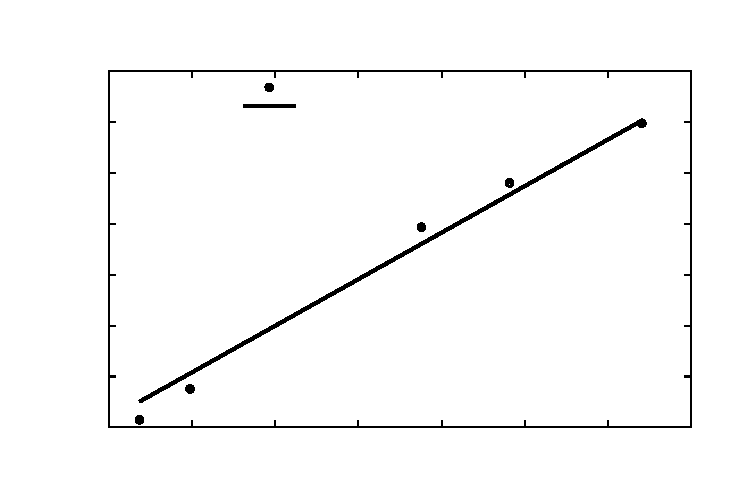
\includegraphics{./../graph/graphB}}%
    \gplfronttext
  \end{picture}%
\endgroup
